\documentclass[10pt,a4paper]{amsart}
\usepackage{amsmath,amssymb,amsthm,graphicx}
% Class-compatibility preamble for a reader excerpt of
%   Masuda-Thomas-Tonks-Vallette, "The diagonal of the associahedra", JEP 8 (2021), DOI 10.5802/jep.142.
%
% This file is the source directory's inherited layout adapter, unchanged except for one
% mechanical line: \smaller is declared with \providecommand instead of \newcommand because the
% wrapper class used for this excerpt (amsart) already defines \smaller as a font-size command.
% No mathematical macro, statement or proof step is added.
\usepackage{amsmath,amssymb,amsthm,xfrac,xspace,hyperref,graphicx,comment}
\excludecomment{DefTralics}

\providecommand{\bibliofont}{\small}
\newcommand{\ie}{i.e.,\xspace}
\newcommand{\eg}{e.g.,\xspace}
\newcommand{\etc}{etc.\xspace}
\newcommand{\cf}{cf.\xspace}
\newcommand{\resp}{resp.\xspace}
\providecommand{\smaller}{\small}
\newcommand{\Subsection}{\subsection}
\newcommand{\Subsubsection}{\subsubsection}
\newcommand{\skpt}{\smallskip}
\emergencystretch=3em
\numberwithin{equation}{section}\providecommand{\No}{}
\usepackage{mathrsfs}
\let\mathcal\mathscr
\usepackage{mathtools}
\newcommand{\Changel}{\mathcode`l="7160}
\newcommand{\Changelback}{\mathcode`l="716C}
\newcommand{\NoChangel}[1]{%
\expandafter\let\csname old\string#1\endcsname=#1
\let#1=\relax
\newcommand{#1}{\mathcode`l="716C\csname old\string#1\endcsname\mathcode`l="7160 }%
}
\def\mto{\mathchoice{\longmapsto}{\mapsto}{\mapsto}{\mapsto}}
\def\hto{\mathrel{\lhook\joinrel\to}}
\def\ltwoheadrightarrow{\longrightarrow\hspace*{-5mm}\longrightarrow}
\def\stwoheadrightarrow{\rightarrow\hspace*{-3mm}\rightarrow}
\def\twoheadrightarrow{\mathchoice{\ltwoheadrightarrow}{\stwoheadrightarrow}{\stwoheadrightarrow}{\stwoheadrightarrow}}
\def\To#1{\mathchoice{\xrightarrow{\textstyle\kern4pt#1\kern3pt}}{\stackrel{#1}{\longrightarrow}}{}{}}
\def\Hto#1{\mathrel{\lhook\joinrel\To{#1}}}
\newcommand{\sbullet}{{\scriptscriptstyle\bullet}}

\NoChangel{\log}
\NoChangel{\ln}
\NoChangel{\lim}
\NoChangel{\limsup}
\NoChangel{\liminf}
\NoChangel{\varlimsup}
\NoChangel{\varliminf}
\NoChangel{\varinjlim}
\NoChangel{\varprojlim}

\let\dpl\displaystyle
\let\ts\textstyle

\AtBeginDocument{%
\def\labelitemi{$\sbullet$}%
}

\usepackage{graphicx}
\usepackage{multirow}

\usepackage[noabbrev,capitalize]{cleveref}
\crefdefaultlabelformat{#2\textup{#1}#3}

\usepackage{tikz}
\usepackage{tikz-cd}
\tikzset{math3d/.style=
{x= {(-0.353cm,-0.353cm)}, z={(0cm,1cm)},y={(1cm,0cm)}}}
\tikzset{JLL3d/.style=
{x= {(0.4cm,-0.2cm)}, z={(0cm,1cm)},y={(-1cm,0cm)}}}

\theoremstyle{plain}
\newtheorem{proposition}{Proposition}
\newtheorem{theorem}{Theorem}
\newtheorem*{problem}{Problem}
\newtheorem{corollary}{Corollary}
\newtheorem{lemma}{Lemma}
\newtheorem{conjecture}{Conjecture}

\theoremstyle{definition}
\newtheorem{definition}{Definition}
\newtheorem{remark}{Remark}
\newtheorem{example}{Example}

\newcommand{\RR}{\mathbb{R}}
\newcommand{\ZZ}{\mathbb{Z}}
\newcommand{\ZP}{\mathbb{Z}_{>0}}
\newcommand{\K}{{K}}
\newcommand{\La}{\mathcal{L}}
\newcommand{\Tam}[1]{\mathrm{PBT}_{#1}}
\newcommand{\PT}[1]{\mathrm{PT}_{#1}}
\newcommand{\sC}{\mathcal{C}}
\newcommand{\PolySub}{\mathsf{Poly}}\NoChangel{\PolySub}
\newcommand{\Top}{\mathsf{Top}}
\newcommand{\CW}{\mathsf{CW}}
\newcommand{\sF}{\mathcal{F}}
\DeclareMathOperator{\tp}{top}
\DeclareMathOperator{\bm}{bot}
\DeclareMathOperator{\pr}{pr}
\DeclareMathOperator{\conv}{conv}
\DeclareMathOperator{\diam}{diam}
\newcommand{\ang}[1]{\langle #1\rangle}
\renewcommand{\No}{\mathcal{N}}
\newcommand{\Ve}{\mathcal{V}}
\newcommand{\Bool}[1]{\{0, 1\}^{#1}}
\newcommand{\sk}{\mathrm{sk}}
\DeclareMathOperator{\vol}{vol}\NoChangel{\vol}
\newcommand{\tr}{\mathrm{tr}}
\newcommand{\id}{\mathrm{id}}
\newcommand{\itd}[1]{\triangle^{(#1)}}
\DeclareMathOperator*{\colim}{\mathrm{colim}}
\DeclareMathOperator{\im}{\mathrm{Im}}
\newcommand{\abs}[1]{\lvert #1\rvert}
\DeclareMathOperator{\codim}{codim}

\newcommand{\TreeR}
{\vcenter{\hbox{
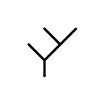
\begin{tikzpicture}[yscale=0.2,xscale=0.2]
\draw[thick] (0,-1)--(0,0) -- (2,2);
\draw[thick] (1,1)--(0,2) ;
\draw[thick] (0,0)--(-1,1) ;
\draw [fill] (0,-1) circle [radius=0.035];
\draw [fill] (2,2) circle [radius=0.035];
\draw [fill] (0,2) circle [radius=0.035];
\draw [fill] (-1,1) circle [radius=0.035];
\end{tikzpicture}}}}
\newcommand{\TreeL}
{\vcenter{\hbox{
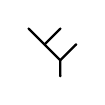
\begin{tikzpicture}[yscale=0.2,xscale=0.2]
\draw[thick] (0,-1)--(0,0) -- (-2,2);
\draw[thick] (-1,1)--(0,2) ;
\draw[thick] (0,0)--(1,1) ;
\draw [fill] (0,-1) circle [radius=0.035];
\draw [fill] (-2,2) circle [radius=0.035];
\draw [fill] (0,2) circle [radius=0.035];
\draw [fill] (1,1) circle [radius=0.035];
\end{tikzpicture}}}}
\newcommand{\TreeLL}
{\vcenter{\hbox{
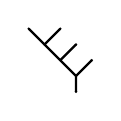
\begin{tikzpicture}[yscale=0.2,xscale=0.2]
\draw[thick] (0,-1)--(0,0) -- (-3,3);
\draw[thick] (-1,1)--(0,2) ;
\draw[thick] (-2,2)--(-1,3) ;
\draw[thick] (0,0)--(1,1) ;
\draw [fill] (0,-1) circle [radius=0.035];
\draw [fill] (-2,2) circle [radius=0.035];
\draw [fill] (0,2) circle [radius=0.035];
\draw [fill] (1,1) circle [radius=0.035];
\draw [fill] (-3,3) circle [radius=0.035];
\draw [fill] (-1,3) circle [radius=0.035];
\end{tikzpicture}}}}
\newcommand{\TreeLR}
{\vcenter{\hbox{
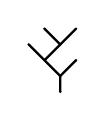
\begin{tikzpicture}[yscale=0.2,xscale=0.2]
\draw[thick] (0,-1)--(0,0) -- (-2,2);
\draw[thick] (-1,1)--(1,3) ;
\draw[thick] (0,0)--(1,1) ;
\draw[thick] (0,2)--(-1,3) ;
\draw [fill] (0,-1) circle [radius=0.035];
\draw [fill] (-2,2) circle [radius=0.035];
\draw [fill] (0,2) circle [radius=0.035];
\draw [fill] (1,1) circle [radius=0.035];
\draw [fill] (-1,3) circle [radius=0.035];
\draw [fill] (1,3) circle [radius=0.035];
\end{tikzpicture}}}}
\newcommand{\TreeRR}
{\vcenter{\hbox{
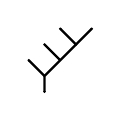
\begin{tikzpicture}[yscale=0.2,xscale=0.2]
\draw[thick] (0,-1)--(0,0) -- (3,3);
\draw[thick] (1,1)--(0,2) ;
\draw[thick] (2,2)--(1,3) ;
\draw[thick] (0,0)--(-1,1) ;
\draw [fill] (0,-1) circle [radius=0.035];
\draw [fill] (2,2) circle [radius=0.035];
\draw [fill] (0,2) circle [radius=0.035];
\draw [fill] (-1,1) circle [radius=0.035];
\draw [fill] (3,3) circle [radius=0.035];
\draw [fill] (1,3) circle [radius=0.035];
\end{tikzpicture}}}}
\newcommand{\TreeRL}
{\vcenter{\hbox{
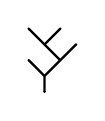
\begin{tikzpicture}[yscale=0.2,xscale=0.2]
\draw[thick] (0,-1)--(0,0) -- (2,2);
\draw[thick] (1,1)--(-1,3) ;
\draw[thick] (0,0)--(-1,1) ;
\draw[thick] (0,2)--(1,3) ;
\draw [fill] (0,-1) circle [radius=0.035];
\draw [fill] (2,2) circle [radius=0.035];
\draw [fill] (0,2) circle [radius=0.035];
\draw [fill] (-1,1) circle [radius=0.035];
\draw [fill] (1,3) circle [radius=0.035];
\draw [fill] (-1,3) circle [radius=0.035];
\end{tikzpicture}}}}
\newcommand{\TreeCC}
{\vcenter{\hbox{
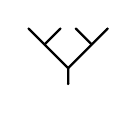
\begin{tikzpicture}[yscale=0.2,xscale=0.2]
\draw[thick] (0,-1)--(0,0) -- (-2.5,2.5);
\draw[thick] (-1.5,1.5)--(-0.5,2.5) ;
\draw[thick] (1.5,1.5)--(0.5,2.5) ;
\draw[thick] (0,0)--(2.5,2.5) ;
\draw [fill] (0,-1) circle [radius=0.035];
\draw [fill] (-2.5,2.5) circle [radius=0.035];
\draw [fill] (-0.5,2.5) circle [radius=0.035];
\draw [fill] (0.5,2.5) circle [radius=0.035];
\draw [fill] (2.5,2.5) circle [radius=0.035];
\end{tikzpicture}}}}
\newcommand{\TreeAL}
{\vcenter{\hbox{
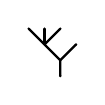
\begin{tikzpicture}[yscale=0.2,xscale=0.2]
\draw[thick] (0,-1)--(0,0) -- (-2,2);
\draw[thick] (-1,1)--(0,2) ;
\draw[thick] (0,0)--(1,1) ;
\draw[thick] (-1,1)--(-1,2) ;
\draw [fill] (0,-1) circle [radius=0.035];
\draw [fill] (-2,2) circle [radius=0.035];
\draw [fill] (0,2) circle [radius=0.035];
\draw [fill] (1,1) circle [radius=0.035];
\draw [fill] (-1,2) circle [radius=0.035];
\end{tikzpicture}}}}
\newcommand{\TreeRA}
{\vcenter{\hbox{
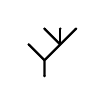
\begin{tikzpicture}[yscale=0.2,xscale=0.2]
\draw[thick] (0,-1)--(0,0) -- (2,2);
\draw[thick] (1,1)--(0,2) ;
\draw[thick] (0,0)--(-1,1) ;
\draw[thick] (1,1)--(1,2) ;
\draw [fill] (0,-1) circle [radius=0.035];
\draw [fill] (2,2) circle [radius=0.035];
\draw [fill] (0,2) circle [radius=0.035];
\draw [fill] (-1,1) circle [radius=0.035];
\draw [fill] (1,2) circle [radius=0.035];
\end{tikzpicture}}}}
\newcommand{\TreeAR}
{\vcenter{\hbox{
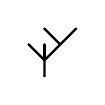
\begin{tikzpicture}[yscale=0.2,xscale=0.2]
\draw[thick] (0,-1)--(0,0) -- (2,2);
\draw[thick] (1,1)--(0,2) ;
\draw[thick] (0,0)--(-1,1) ;
\draw[thick] (0,0)--(0,1) ;
\draw [fill] (0,-1) circle [radius=0.035];
\draw [fill] (2,2) circle [radius=0.035];
\draw [fill] (0,2) circle [radius=0.035];
\draw [fill] (-1,1) circle [radius=0.035];
\draw [fill] (0,1) circle [radius=0.035];
\end{tikzpicture}}}}
\newcommand{\TreeLA}
{\vcenter{\hbox{
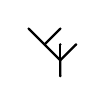
\begin{tikzpicture}[yscale=0.2,xscale=0.2]
\draw[thick] (0,-1)--(0,0) -- (-2,2);
\draw[thick] (-1,1)--(0,2) ;
\draw[thick] (0,0)--(1,1) ;
\draw[thick] (0,0)--(0,1) ;
\draw [fill] (0,-1) circle [radius=0.035];
\draw [fill] (-2,2) circle [radius=0.035];
\draw [fill] (0,2) circle [radius=0.035];
\draw [fill] (1,1) circle [radius=0.035];
\draw [fill] (0,1) circle [radius=0.035];
\end{tikzpicture}}}}
\newcommand{\TreeCA}
{\vcenter{\hbox{
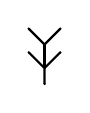
\begin{tikzpicture}[yscale=0.2,xscale=0.2]
\draw[thick] (0,-1)--(0,0) -- (-1,1);
\draw[thick] (0,1.5)--(1,2.5) ;
\draw[thick] (0,1.5)--(-1,2.5) ;
\draw[thick] (0,0)--(1,1) ;
\draw[thick] (0,0)--(0,1.5) ;
\draw [fill] (0,-1) circle [radius=0.035];
\draw [fill] (-1,1) circle [radius=0.035];
\draw [fill] (1,2.5) circle [radius=0.035];
\draw [fill] (-1,2.5) circle [radius=0.035];
\draw [fill] (1,1) circle [radius=0.035];
\draw [fill] (0,1) circle [radius=0.035];
\end{tikzpicture}}}}
\newcommand{\TreeC}
{\vcenter{\hbox{
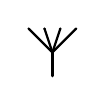
\begin{tikzpicture}[yscale=0.2,xscale=0.2]
\draw[thick] (0,-1.5)--(0,0);
\draw[thick] (0,0)--(1.5,1.5) ;
\draw[thick] (0,0)--(0.5,1.5) ;
\draw[thick] (0,0)--(-0.5,1.5) ;
\draw[thick] (0,0)--(-1.5,1.5) ;
\draw [fill] (0,-1.5) circle [radius=0.035];
\draw [fill] (1.5,1.5) circle [radius=0.035];
\draw [fill] (0.5,1.5) circle [radius=0.035];
\draw [fill] (-1.5,1.5) circle [radius=0.035];
\draw [fill] (-0.5,1.5) circle [radius=0.035];
\end{tikzpicture}}}}
\title{Monotonicity, positivity, edge direction and facet containment for the folding map of the associahedron}
\author{Naruki Masuda, Hugh Thomas, Andy Tonks, Bruno Vallette}
\date{doi:10.5802/jep.142; CC BY 4.0}
\begin{document}
\maketitle
\noindent\textit{Editorial note.} All delivered mathematical text is the author's own, copied from the pinned publisher source sources/jep-2021-142-associahedra-diagonal/full-original-native.tex; no statement or proof step was rewritten, reordered or removed.\par\medskip
\noindent\textit{Editorial note.} Preamble provenance: the retained preamble is the source's own retained-preamble.tex (the class-compatibility file prepared for this source, with \textbackslash{}smaller declared by \textbackslash{}providecommand) plus the author's macro block at lines 39-303 of sources/jep-2021-142-associahedra-diagonal/full-original-native.tex (everything from the author's first package to the line before \textbackslash{}begin\{document\}, comments excluded; the publisher class, its private \textbackslash{}makeatletter block and the conditional font-shape rule are left out deliberately). Nothing was added, no macro was invented, and the excerpt serves only as preamble, never as a span coordinate.\par\medskip
\noindent\textit{Editorial note.} Assembly history: the first attempt (r001) used inherited-layout-adapter.tex, whose \textbackslash{}newcommand\{\textbackslash{}smaller\}\{\textbackslash{}small\} clashes with the amsart wrapper (LaTeX error: command \textbackslash{}smaller already defined); r002 switches to the source's retained-preamble.tex, which is the same adapter with \textbackslash{}providecommand, and to the author block starting at the first package line. No mathematical text changed between the revisions.\par\medskip
\noindent\textit{Editorial note.} External references are navigation pointers only; every deliberately kept step of the author's argument stays inside the counted spans. The displayed numbers of those pointers are the author's own numbering under the author's \textbackslash{}newtheorem declarations (section.index as declared), computed mechanically by the lane's scanner.\par\medskip
\noindent\textit{Editorial note.} Clause (2) of the statement is dismissed by the author with 'This is straightforward from the definition of v' (proof line 1432); the other three clauses carry their own arguments inside the counted span. The sentence is kept verbatim.\par\medskip
\noindent\textit{Editorial note.} The proof reads the clauses in the statement's own order and needs no reference to any item outside the counted range, so no navigation stub was required.\par\medskip
\noindent\textit{Allowed standard prerequisites (editorial).}\begin{itemize}
\item The folding map L from the vertices of the polytope P onto the Boolean lattice, and the vector v defined from the sequence a\_i. Set up immediately before the counted statement, in the paragraph ending at source line 1412. Supplies the objects L, v and the increasing sequence a\_i in terms of which all four clauses are phrased.
\item The adjacencies of the associahedron are generated by rotating pairs of successive left- and right-leaning edges. Used inside the counted proof at lines 1430 and 1434-1438. Lets the author compare two neighbouring trees s and t and compute the edge vector between their images.
\end{itemize}\medskip
\begin{lemma}\label{lemma:propertiesofL}
The following properties are satisfied:
\begin{enumerate}
\item\label{lemma:propertiesofL1} $s\leq t$ $\Rightarrow L(s)\leq L(t)$,

\item\label{lemma:propertiesofL2} $\ang{\vec e_i, \vec v} >0$, for $1\leq i \leq d$,

\item\label{lemma:propertiesofL3} each edge connecting $s\in L^{-1}_i (0)$ and $t\in L^{-1}_i(1)$ is parallel to $\vec e_i$,

\item\label{lemma:propertiesofL4} any fiber $L^{-1}(b)$, for $b\in \Bool{d}$, is contained in a facet of $P$.
\end{enumerate}
\end{lemma}

\begin{proof}
\begin{enumerate}
\item When we switch a pair of successive left and right-leaning edges to a pair of successive right and left-leaning edges, either it does not change the orientation of the leaves or it just changes one left-leaning leaf into a right-leaning leaf.

\item This is straightforward from the definition of $\vec v$.

\item It is enough to prove it on one polytope $K_\omega$.
In this case, $t$ is a planar binary tree obtained from a planar binary tree $s$ by switching the $(i+1)^\text{th}$ leaf from left-leaning to right-leaning, which implies
\[
\overrightarrow{M(s, \omega)M(t, \omega)}=\omega_i\omega_{i+2}\vec e_i.
\]
\item Reading the sequence $(1, b_1, \ldots, b_{n_1-2}, 0)$ from left to right, there is at least one occurrence of $(1,0)$, say at place $i$ and $i+1$. Every face labeled by a forest of trees~$t$ satisfying $L(t)=b$ lies in the facet labeled by $\big(c_{n_1-1}\circ_i c_2, c_{n_2}, \ldots, c_{n_k}\big)$.\qedhere
\end{enumerate}
\end{proof}

\begin{thebibliography}{99}
\bibitem{AguiarArdila17} M. Aguiar \& F. Ardila - “Hopf monoids and generalized permutahedra” , 2017
\bibitem{Amorim17} L. Amorim - “The Künneth theorem for the Fukaya algebra of a product of Lagrangians” , Internat. J. Math. 28 (2017) no. 4, article ID 1750026, 38 pages
\bibitem{Brown59} E. H. Brown - “Twisted tensor products. I” , Ann. of Math. (2) 69 (1959), p. 223-246
\bibitem{BilleraSturmfels92} L. J. Billera \& B. Sturmfels - “Fiber polytopes” , Ann. of Math. (2) 135 (1992) no. 3, p. 527-549
\bibitem{BoardmanVogt73} J. M. Boardman \& R. M. Vogt - Homotopy invariant algebraic structures on topological spaces , Lect. Notes in Math. , vol. 347 , Springer-Verlag, Berlin, 1973
\bibitem{CFZ02} F. Chapoton, S. Fomin \& A. Zelevinsky - “Polytopal realizations of generalized associahedra” , Canad. J. Math. 45 (2002) no. 4, p. 537-566
\bibitem{CSZ15} C. Ceballos, F. Santos \& G. M. Ziegler - “Many non-equivalent realizations of the associahedron” , Combinatorica 35 (2015) no. 5, p. 513-551
\bibitem{EilenbergMacLane54} S. Eilenberg \& S. Mac Lane - “On the groups $H(\Pi ,n)$. II. Methods of computation” , Ann. of Math. (2) 60 (1954), p. 49-139
\bibitem{EilenbergZilber53} S. Eilenberg \& J. A. Zilber - “On products of complexes” , Amer. J. Math. 75 (1953), p. 200-204
\bibitem{Forcey08} S. Forcey - “Convex hull realizations of the multiplihedra” , Topology Appl. 156 (2008) no. 2, p. 326-347
\bibitem{GKZ08} I. M. Gelfand, M. M. Kapranov \& A. V. Zelevinsky - Discriminants, resultants and multidimensional determinants , Modern Birkhäuser Classics , Birkhäuser Boston, Inc., Boston, MA, 2008
\bibitem{GaberdielZwiebach97} M. R. Gaberdiel \& B. Zwiebach - “Tensor constructions of open string theories. I. Foundations” , Nuclear Phys. B 505 (1997) no. 3, p. 569-624
\bibitem{Loday04a} J.-L. Loday - “Realization of the Stasheff polytope” , Arch. Math. (Basel) 83 (2004) no. 3, p. 267-278
\bibitem{LodayVallette12} J.-L. Loday \& B. Vallette - Algebraic operads , Grundlehren Math. Wiss. , vol. 346 , Springer-Verlag, Berlin, 2012
\bibitem{May72} J. May - The geometry of iterated loop spaces , Lect. Notes in Math. , vol. 271 , Springer-Verlag, Berlin, 1972
\bibitem{MarklShnider06} M. Markl \& S. Shnider - “Associahedra, cellular $W$-construction and products of $A_\infty $-algebras” , Trans. Amer. Math. Soc. 358 (2006) no. 6, p. 2353-2372
\bibitem{MSS} M. Markl, S. Shnider \& J. D. Stasheff - Operads in algebra, topology and physics , Math. Surveys and Monographs , vol. 96 , American Mathematical Society, Providence, RI, 2002
\bibitem{Proute11} A. Prouté - “$A_\infty $-structures. Modèles minimaux de Baues-Lemaire et Kadeishvili et homologie des fibrations” , Repr. Theory Appl. Categ. (2011) no. 21, p. 1-99, Reprint of the 1986 original, With a preface to the reprint by Jean-Louis Loday
\bibitem{Seidel08} P. Seidel - Fukaya categories and Picard-Lefschetz theory , Zürich Lectures in Advanced Math. , European Mathematical Society, Zürich, 2008
\bibitem{Serre51} J.-P. Serre - “Homologie singulière des espaces fibrés. Applications” , Ann. of Math. (2) 54 (1951), p. 425-505
\bibitem{StasheffShnider97} J. D. Stasheff \& S. Shnider - “From operads to “physically” inspired theories (Appendix B)” , in Operads: Proceedings of Renaissance Conferences (Hartford, CT/Luminy, 1995) , Contemp. Math. , vol. 202 , American Mathematical Society, Providence, RI, 1997, p. 53-81
\bibitem{Stasheff63} J. D. Stasheff - “Homotopy associativity of $H$-spaces. I \& II” , Trans. Amer. Math. Soc. 108 (1963), p. 275-292 \& 293–312
\bibitem{Stasheff70} J. D. Stasheff - $H$-spaces from a homotopy point of view , Lect. Notes in Math. , vol. 161 , Springer-Verlag, Berlin, 1970
\bibitem{Steenrod47} N. E. Steenrod - “Products of cocycles and extensions of mappings” , Ann. of Math. (2) 48 (1947), p. 290-320
\bibitem{SaneblidzeUmble04} S. Saneblidze \& R. Umble - “Diagonals on the permutahedra, multiplihedra and associahedra” , Homology Homotopy Appl. 6 (2004) no. 1, p. 363-411
\bibitem{Tamari51} D. Tamari - Monoïdes préordonnés et chaînes de Malcev , Thèse de Mathématique, Paris, 1951
\bibitem{Ziegler95} G. M. Ziegler - Lectures on polytopes , Graduate Texts in Math. , vol. 152 , Springer-Verlag, New York, 1995
\end{thebibliography}
\end{document}
